


\documentclass{beamer}
\usepackage[francais]{babel}
\usepackage[T1]{fontenc}
\usepackage[utf8]{inputenc}     
\usepackage{verbatim}           
\usepackage{graphicx}
\usepackage{array}
\usepackage{color}

\usetheme{Warsaw}
\useoutertheme{infolines}

\graphicspath{{Image/}}
\setbeamertemplate{caption}[numbered]


\title{Réseau de Pert et Diagramme de Gantt}
\author {T.~DeRibas \and A.~Lefevre}
\institute{UM2}
\date{06/02/2017}

\begin{document}




\begin{frame}
  \frametitle{Table des matières}
  { \tableofcontents}
\end{frame}


\section{Introduction}

\begin{frame}
  \frametitle{Introduction}
  \begin{itemize}
  \item Le réseaux de Pert et le diagramme de Gantt sont deux techniques de planification de projet.
  \item Ils sont basés sur une réprésentation graphique et sont complémentaires
  \end{itemize}
\end{frame}


\section{Gantt}

\subsection{Introduction}

\begin{frame}
  \frametitle{Introduction à Gantt}
  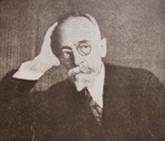
\includegraphics{karol}
  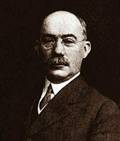
\includegraphics{gant}
 
   
   
  \begin{itemize}
   
  \item Outil de planification des tâches.
  \item Premier réaliser en  1896 par \alert{Karol~Adamiecki}.
  \item Publié en 1910 par \alert{Henry~L.Gantt}.
  \item Aujourd'hui \textbf{les logicels informatiques simplifie grandement leur utilisation}
  \end{itemize}
\end{frame}

\begin{frame}
  \frametitle{Principe d'un diagramme de gantt}
  \begin{itemize}
  \item Il s'agit d'un diagramme avec:
    \begin{itemize}
    \item \textbf{En ordonnée:} La liste des taches du projet.
    \item \textbf{En abscisse:} Une unité de temps (jours , semaines , mois...)
    \end{itemize}
  \item Permet de visualiser simplement les différentes activités d'un projet et leurs échéances.
  \item On peut associer au différentes tâches des ressources, des connexions, des dates.
  \item Facilement mit à jours, \textbf{il est adapté à tous les secteurs} et utilisé par une majorité de chef de projet.
  \end{itemize}
\end{frame}


\begin{frame}
  \begin{figure}
    \centering
    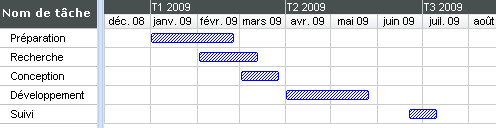
\includegraphics[width=0.8\textwidth]{Sgantt}
    \caption{Un diagramme de Gantt simple}
  \end{figure}
\end{frame}



\begin{frame}
  \frametitle{Intérêt}
  \begin{description}
  \item[Adaptable] \alert{Quelque soit la nature du projet} et les différents domaines impliqué \alert{le diagramme de Gantt est utilisable pour tous les domaines d'activité.}
  \item[Facilite l'organisation] Les taches et leurs difficultés sont représentées par \textbf{des éléments visuels simples.} Ce qui donne une vision complète de la structure du projet avec l'ordre des taches, leurs importances et les dates d'échéances
  \item[Dynamique] A chaque modification de planning, le diagramme \alert{recalcule automatiquement les dates, durées et échéance} de chaque tâche.
  \end{description}
  \begin{block} {Actuellement}
   C'est le moyen le plus efficace pour répertorier les activités nécessaires en vue de mener à bien ses projets.
  \end{block}
\end{frame}


\subsection{Comment créer un diagramme de Gantt}

\begin{frame}
  \frametitle{Comment créer un diagramme de Gantt}
  \begin{itemize}
  \item Plusieurs logiciels disponibles sur le Web. (Ex: Sciforma, GANTTProject)
  \item \alert{Possible de fabriquer un diagramme via un tableur Excel.}
  \item La fabrication d'un diagramme passe par les mêmes phases que l'on peut regrouper en \textbf{5 étapes.}
    \begin{enumerate}[<+-| alert@+>]
    \item Le listing des tâches.
    \item L'attribution des ressources.
    \item La planification dans le temps.
    \item La création des connexions entre les tâches.
    \item L'ajouts des contraintes et des jalons.
    \end{enumerate}
    
  \end{itemize}
\end{frame}


\begin{frame}
  \begin{figure}
    \centering
    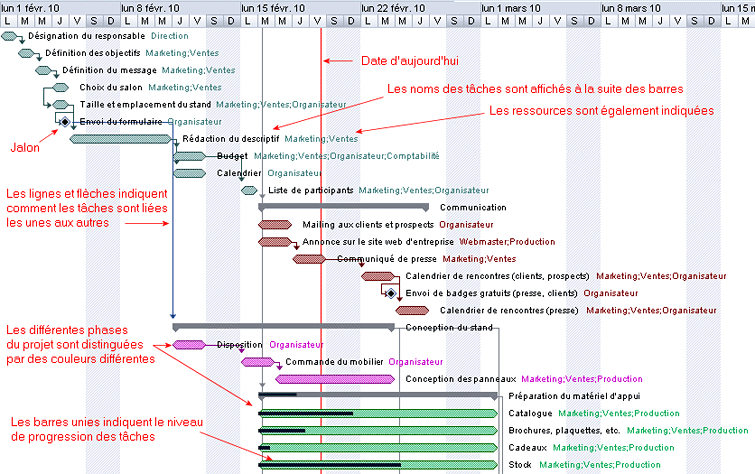
\includegraphics[width=1\textwidth]{Cgantt}
    \caption{Un diagramme de Gantt plus complexe}
  \end{figure}
\end{frame}


\begin{frame}
  \frametitle{Etape 1: Le listing des tâches}
  \begin{itemize}
  \item Dans le cadre de la création d'un diagramme de Gantt, vous devez commencer par \alert{lister toutes les tâches qui devront être accomplies} pour que le projet soit mené à bien.
  \item A chacune de ses tâches peuvent être attribuées des sous-tâches.
  \item \alert{Pensez à tous les éléments}, même les plus insignifiants : un oubli peut retarder toute la réalisation du projet.
  \item Cet ensemble de tâches et sous-tâches hiérarchisées se retrouvera listé à gauche du diagramme.
  \end{itemize}
\end{frame}

\begin{frame}
  \frametitle{Etape 2: L'attribution des ressources.}
  \begin{itemize}
  \item A chaque activité et sous-activité, une ou plusieurs ressources peuvent être affectées.
  \item Les ressources humaines sont représentées sous forme de pourcentage. \textbf{100\% correspond à une personne à temps plein.}
  \item Les matériaux par \alert{leurs quantités ou leur taux de consommation.}
  \item Les couts des ressources peuvent également être indiqué.
  \item Certains logiciels \alert{ajustent automatiquement la longueur} des barres du diagramme selon la quantité de ressources allouées.
  \end{itemize}
\end{frame}


\begin{frame}
  \frametitle{Etape 3: La planification dans le temps.}
  \begin{itemize}
  \item Une fois toutes les tâches référencées, il faut les étaler dans le temps.
  \item \alert{Dater le début du projet}, puis établir un ordre d'exécution des tâches.
  \item \textbf{Primordial pour repérer l'état d'avancement du projet.}
  \end{itemize}
\end{frame}

\begin{frame}
  \frametitle{Etape 4: Les connexion entre les tâches.}
  \begin {itemize}
  \item On retrouve des \textbf{dépendances} dans les taches d'un projet: certaines tâches ne peuvent commencer que si l'une est terminée, par exemple.
  \item Il faut alors \alert{créer des liens} entre les tâches afin de \alert{mieux visualiser} ces connexions qui lieront le projet.
  \item Celle-ci seront matérialisées par \textbf{des flèches} entre chaque rectangle. Et c'est grâce à elle que \textbf{le diagramme devient dynamique.}
  \end{itemize}
\end{frame}

\begin{frame}{Les différents types de liaisons}
  Il existe 4 types de liaisons
  \begin{description}
  \item[Fin à Début(FD)] La tâche\textbf{ ne peut pas commencer} si celle antérieure \textbf{n'est pas terminée}. Elle peut toutefois commencer plus tard. Il s'agit du type de dépendance le plus courant.
  \item[Début à Début(DD)] La tâche \textbf{ne peut pas commencer} si celle antérieure \textbf{n'est pas commencée}. Elle peut toutefois commencer plus tard.
  \item[Fin à Fin(FF)]  La tâche\textbf{ ne peut pas ce terminer} si celle antérieure \textbf{n'est pas terminée}. Elle peut toutefois se terminer plus tard.
  \item[Début à Fin(DF)]  La tâche\textbf{ ne peut pas ce terminer} si celle antérieure \textbf{n'est pas commencée}. Elle peut toutefois se terminer plus tard. Ce type de liaison est rarement utilisé.
  \end{description}
\end{frame}


\begin{frame}
  \begin{figure}
    \centering
    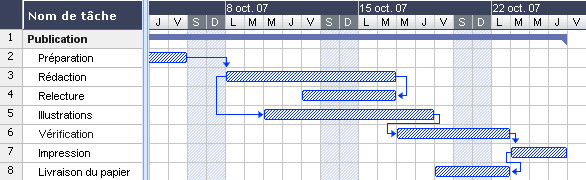
\includegraphics[width=0.8\textwidth]{Dfleche}
    \caption{Les différentes connexions d'un diagramme}
  \end{figure}
\end{frame}



\begin{frame}
  \frametitle{Etape 5: Les contraintes et jalons}
  \begin{block}{Les contraintes}
   Elles permettent d'imposer des dates de début ou de fin a certaines tâches.
   \\ Ces limites réduisent la flexibilité du diagramme, s'il y a opposition entre une contrainte et une connexion le logiciel le marque et donne la priorité à la contrainte.
   \end{block}
 \begin{block}{Le jalon}
   Il indique une date clef du projet, mais ce n'est pas une tâche.
   \\Le jalon scinde le diagramme en plusieurs parties grâce à différentes échéances intermédiaires.
   \\Il peut s'agir de la signature d'un contrat, la publication d'un document
   \\ Il est représenté graphiquement pas un losange.
  \end{block}
  \begin{figure}
    \centering
    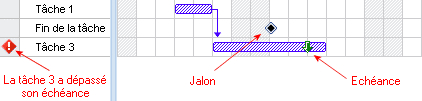
\includegraphics[width=0.55\textwidth]{JC}
  \end{figure}
\end{frame}


\subsection{Suivi du diagramme de Gantt}

\begin{frame}
  \frametitle{Suivi du diagramme de Gantt}
  Une fois votre projet mis au point et démarré, il convient de l'inspecter régulièrement pour détecter les problèmes et conflits éventuels afin de les résoudre en temps utile.
  \begin{itemize}[<+-| alert@+>]
  \item Votre projet se déroule-t-il comme prévu ?
  \item Les liaisons établies entre les tâches sont-elles toutes nécessaires ?
  \item Toutes les contraintes définies ont elles l'effet voulu ?
  \end{itemize}
\end{frame}


  


\section{PERT}

\subsection{Histoire}

\begin{frame}{POLARIS}
  \begin{itemize}
    \item 1957-1958 : la marine Américaine veut mener à son terme le plus rapidement possible le projet \textbf{POLARIS} (sous-marin lance missiles ainsi que ses missiles)
    \item 250 fournisseurs et plus de 9000 sous-traitants : ordonnancement des tâches très complexe
    \item durée du projet prévu \textbf{7 ans}
\end{itemize}
\end{frame}

\begin{frame}{POLARIS II}
\begin{figure}
      \centering
      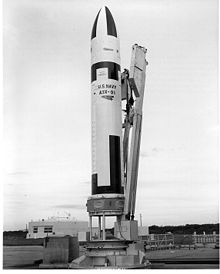
\includegraphics[width=0.3\textwidth]{missile}
      \caption{Missile POLARIS}
\end{figure}
\end{frame}

\begin{frame}{POLARIS III}
\begin{itemize}
    \item Ce sont les ingénieurs du bureau de planning de la marine qui ont mis au point une méthode d'ordonnancement s'appuyant sur les mathématiques modernes
    \item La méthode \textbf{PERT} était née, elle devait permettre un gain de \textbf{deux} ans sur la durée du projet POLARIS
\end{itemize}
\end{frame}

\subsection{Fonctionnement}

\begin{frame}{Quelques notions}
\begin{description}
    \item[Tâche] Une \textbf{tâche} est représentée par une flèche et caractérisée par un \textbf{nom} (A) et une \textbf{durée} (10), elle évolue d'un état initial à un état final 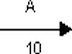
\includegraphics[width=0.1\textwidth]{tache}
    \item[Etape] Une \textbf{étape} (aussi appelée "évènement") est le début (ou la fin) d'une \textbf{tâche}. Elle a un \textbf{numéro} (1), une \textbf{durée minimale} (date au plus tôt) (10) et \textbf{maximale} (date au plus tard) (18) 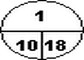
\includegraphics[width=0.1\textwidth]{etape}
    \item[Réseau] Le \textbf{réseau} c'est l'ensemble des \textbf{tâches} et des \textbf{étapes} qui définissent le projet. Il met en évidence les relations entre les tâches et les étapes. 
\end{description}
\end{frame}

\begin{frame}{Quelques notions II}
\begin{figure}
      \centering
      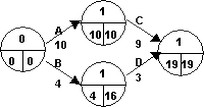
\includegraphics[width=0.5\textwidth]{reseau}
      \caption{Reseau PERT}
\end{figure}
\end{frame}

\begin{frame}{Conventions}
\begin{enumerate}
    \item Toute \textbf{tâche} a pour début une \textbf{étape} d’origine et pour extrémité une \textbf{étape} de fin.
    \item Une \textbf{étape} ne peut être atteinte que lorsque toutes les \textbf{tâches} qui la précèdent sont terminées.
    \item Aucune \textbf{tâche} ne peut être réalisée si l’\textbf{étape} d’origine n’a pas été atteinte.
\end{enumerate}
\end{frame}

\begin{frame}{Principe}
\begin{itemize}
    \item Réalisation d'un projet : exécution de tâches dans un ordre donné en tenant compte des \textbf{relations} existantes entre elles
    \item Ces \textbf{relations} sont de deux ordres : 
    \begin{itemize}
        \item \textbf{Relations logiques} : on ne peut pas commencer une tâche avant que la précédente ne soit terminée (ex : compiler un programme avant de l'exécuter)
        \item \textbf{Relations d'ordre spéculatif} : l'enchainement des tâches est alors défini par contraintes (moyen ou délai)
    \end{itemize}
    
\end{itemize}
\end{frame}

\begin{frame}{Préliminaires}
\begin{block}{Renseignement sur les tâches}
\begin{tabular}{|c|c|c|c|c|}
\hline
    / & Désignation & Durée (jours) & Tâche(s) antérieure(s) \\
    \hline
    A & Définition du budget & 4 & / \\
    \hline
    B & Sélection thème, date, lieu & 3 & A \\
    \hline
    C & Embauche traiteur & 3 & B \\
    \hline
    D & Annonce interne & 3 & B \\
    \hline
    E & Annonce de presse & 4 & D \\
    \hline
    F & Sélection menu & 2 & C \\
    \hline
    G & Location des équipements & 4 & C et E \\
    \hline
    H & Embauche personnel & 4 & G \\
    \hline
    I & Préparatifs & 5 & G \\
    \hline
    J & Evènement & 1 & I, H et F \\
    \hline
\end{tabular}
\end{block}
\end{frame}

\begin{frame}{Préliminaires II}
\begin{block}{Dessin du graphe}
\begin{itemize}
    \item Projet simple : on trace directement le réseau PERT
    \item Projet plus complexe : on utilise une grille (ou matrice). Pour cela, il suffit de prendre la liste des tâches, ligne par ligne, de suivre sur la matrice les lignes correspondant aux opérations et de mettre une croix dans la colonne correspondant à l’opération qui doit avoir lieu avant.
\end{itemize}
\end{block}
\end{frame}

\begin{frame}{Préliminaires III}
\begin{block}{Grille}
\centering
\begin{tabular}{|c|c|c|c|c|c|c|c|c|c|}
\hline
    / & A & B & C & D & E & F & G & H & I \\
    \hline
    A &-&&&&&&&& \\
    \hline
    B &\textcolor{red}{X}&-&&&&&&&\\
    \hline
    C &&\textcolor{red}{X}&-&&&&&&\\
    \hline
    D &&\textcolor{red}{X}&&-&&&&&\\
    \hline
    E &&&\textcolor{red}{X}&&-&&&&\\
    \hline
    F &&&&&\textcolor{red}{X}&-&&&\\
    \hline
    G &&&&&&\textcolor{red}{X}&-&&\\
    \hline
    H &&&&\textcolor{red}{X}&&&&-&\\
    \hline
    I &&&&&&&\textcolor{red}{X}&\textcolor{red}{X}&-\\
    \hline
\end{tabular}
\end{block}
\end{frame}

\begin{frame}{Graphe de liaisons}
\begin{figure}
      \centering
      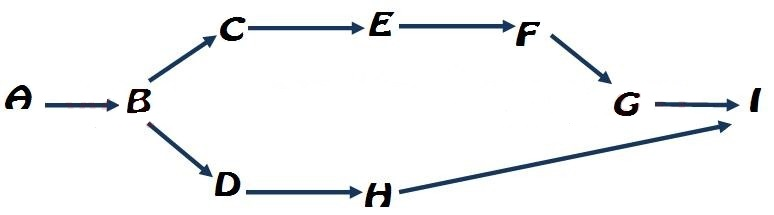
\includegraphics[width=0.5\textwidth]{graphe_liaisons}
      \caption{Graphe de liaisons}
\end{figure}
\end{frame}

\begin{frame}{Construction}
    \begin{itemize}
    \item Maintenant que l'on a construit un réseau correct, c'est à dire que chaque étape est reliée à une autre étape par une tâche.
    \item Connaissant la durée de chaque tâche, il nous est possible de calculer le délai total d’exécution de l’ouvrage, en procédant étape par étape.
        \end{itemize}
\begin{block}{Date au plus tôt}
Date à laquelle une étape peut être franchie. 
\end{block}
\end{frame}

\begin{frame}{Exemple réseau}
\begin{figure}
      \centering
      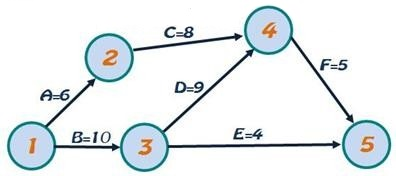
\includegraphics[width=0.5\textwidth]{ex_reseau}
      \caption{ Exemple réseau PERT simple}
\end{figure}
\end{frame}

\begin{frame}{Exemple réseau min}
\begin{block}{Date au plus tôt}
\centering
\begin{tabular}{|c|c|c|}
\hline
    Etape & Opération à considérer & Date au plus tôt \\
    \hline
    1 & / & 0 \\
    \hline
    2 & A & 6 \\
    \hline
    3 & B & 10 \\
    \hline
    4 & C et D & 10+9=19 \\
    \hline
    5 & E et F & 10+9+5=24 \\
    \hline
\end{tabular}
\end{block}
\end{frame}

\begin{frame}{Construction II}
\begin{block}{Date au plus tard}
Date à laquelle une étape doit être atteinte. Elle est obtenue en partant du temps maximal autorisé. Quand plusieurs chemins sont possibles, il faut retenir la date limite la plus petite.
\end{block}
\end{frame}

\begin{frame}{Exemple réseau}
\begin{figure}
      \centering
      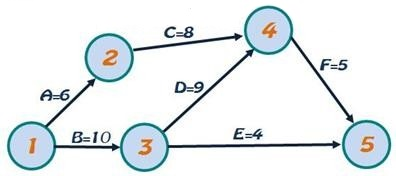
\includegraphics[width=0.5\textwidth]{ex_reseau}
      \caption{ Exemple réseau PERT simple}
\end{figure}
\end{frame}

\begin{frame}{Exemple réseau max}
\begin{block}{Date au plus tard}
\centering
\begin{tabular}{|c|c|c|}
\hline
    Etape & Opération à considérer & Date au plus tard \\
    \hline
    5 & / & 25 (délai total) \\
    \hline
    4 & F & 25-5=20 \\
    \hline
    3 & D et E & 25-5-9=11 \\
    \hline
    2 & C & 25-5-8=12 \\
    \hline
    1 & A et B & 25-5-9-10=1 \\
    \hline
\end{tabular}
\end{block}
\end{frame}

\begin{frame}{Exemple étape}
\begin{figure}
      \centering
      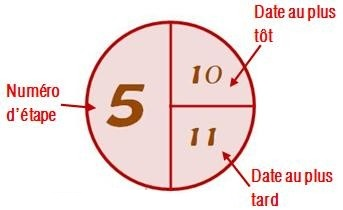
\includegraphics[width=0.5\textwidth]{etape2}
      \caption{ Exemple étape}
\end{figure}
\end{frame}

\begin{frame}{Chemin critique}
\begin{block}{Chemin critique}
C’est le chemin dont la succession des tâches donne la durée d’exécution la plus longue et fournit le délai d'aboutissement du projet. C'est à dire que tout retard prit sur une étape du chemin critique, répercute ce retard sur la durée totale du projet. Il est donc primordial de veiller au bon déroulement des étapes sur ce chemin. Cependant, dans la pratique, il ne représente que 15 à 20\% des étapes du projet.
\end{block}
\end{frame}

\begin{frame}{Exemple réseau critique}
\begin{figure}
      \centering
      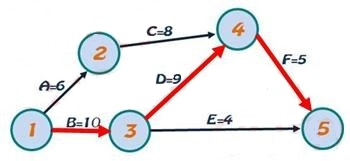
\includegraphics[width=0.5\textwidth]{chemin_critique}
      \caption{ Exemple réseau PERT simple}
\end{figure}
\end{frame}



\section{Conclusion}

\begin{frame}{Conclusion}
    \begin{itemize}
        \item Outils les plus répendus pour planifier un projet, et optimiser l'ordonnancement des tâches à effectuer.
        \item Long à manipuler à la main -> logiciels plus adaptés (MS Project, DotProject, GANTTProject...)
        \item Bien que ces methodes se complètent, leur utilisation ne garentise pas pour autant la réussite du projet...  
    \end{itemize}
\end{frame}

\begin{frame}
\centering
    Merci pour votre écoute !
\end{frame}
\begin{frame}{pour plus d'information}
    \begin{thebibliography}{10}
    
    \beamertemplatebookbibitems   

    \bibitem{Wikipedia}
    Wikipedia
    
    \beamertemplatearticlebibitems
    \bibitem{}
   http://www.Gantt.com
    \bibitem{}
   http://www.diagramme-de-gantt.fr
    \bibitem{} http://www.rocdacier.com/ressource.n.79/cours-sur-le-reseau-pert-methode-pert-.html
    \bibitem{} http://www.prismconseil.fr/site/index.php/planification/La-methode-PERT.html
\end{thebibliography}
\end{frame}

  



\end{document}



